\chapter{Wprowadzenie}

\emph{Grieg} to stworzony w języku Java, kompatybilny z platformą \textit{Android} framework
umożliwiający odczyt i analizę plików dźwiękowych. Powstał w dużej mierze na potrzeby aplikacji do
analizy muzyki, wiele decyzji projektowych jest w związku z tym nastawionych na ułatwienie jego
użycia w sposób interaktywny, łatwo ,,obserwowalny'' dla kodu zewnętrznego.

Nazwa pochodzi od Edwarda Griega –- XIX-wiecznego norweskiego kompozytora romantycznego, twórcy
m.in.  słynnego koncertu fortepianowego \textit{a-moll} oraz suit \textit{Peer Gynt}.

\chapter{Podstawowe operacje}

\section{Wczytanie pliku}

Aby wczytać plik, niezbędne jest posiadanie obiektu klasy \code{FileLoader}. Jeden \code{FileLoader}
służyć może do wczytania dowolnej ilości plików. Wszelki dostęp do pliku dźwiękowego następuje
poprzez obiekt klasy \code{AudioFile}. Utworzyć można go za pomocą metody \code{loadFile(File)}
klasy \code{FileLoader}.  Poniższy fragment kodu stanowi przykład wczytania pliku
\code{music/traumarei.mp3}:

\begin{java}
FileLoader loader = new FileLoader();
File file = new File("./music/traumarei.mp3");
try {
    AudioFile audioFile = loader.loadFile(file);
} catch (NoSuitableDecoderException e) {
    // unknown file format
} catch (IOException e) {
    // problem with file
}
\end{java}

Obecnie obsługiwane są następujące formaty:

\begin{itemize}
  \item mp3
  \item wav
  \item ogg vorbis
\end{itemize}

Jeśli format podanego pliku nie jest wspierany przez framework, metoda \code{loadFile} rzuca wyjątek
typu \code{NoSuitableDecoderException}. W przypadku wystąpienia innych problemów (np.  nieprawidłowa
nazwa pliku), rzucany jest wyjątek \code{IOException}. Samo załadowanie pliku sprawdza poprawność
jedynie począkowego jego fragmentu, zatem przebiega stosunkowo szybko, niezależnie od wielkości
pliku.

\begin{Tip}
Rodzaj pliku jest rozpoznawany po rozszerzeniu, jednak w przypadku, gdy plik o danym rozszerzeniu
nie zawiera prawidłowych dla odpowiadającego mu formatu danych, podejmowana jest próba interpretacji
jego zawartości jako danych w innym formacie. W efekcie plik zostanie poprawnie otwarty, jeśli to
tylko możliwe. Wystąpić mogą jednak problemy z niektórymi metadanymi.
\end{Tip}

\begin{Note}
Możliwe jest dodawanie własnych parserów plików, obsługujących inne formaty. Listę rozszerzeń
obsługiwanych przez konkretny obiekt \code{FileLoader} pobrać można przy użyciu metody
\code{getKnownExtensions()}.
\end{Note}


\section{Dostęp do metadanych}

Po wczytaniu pliku możemy uzyskać dostęp do jego metadanych –- różnych informacji o pliku i jego
zwartości, takich jak czas trwania, tytuł, wykonawca itd. Poszczególne formaty plików różnią się
obsługą tego typu danych (np. tagi ID3 w mp3, tzw. ,,komentarze'' w plikach vorbis), jak również
nazwami poszczególnych informacji, jednak \emph{Grieg} udostępnia metadane przez warstwę abstrakcji,
która ukrywa związane z ich specyfiką szczegóły.

Wspierane przez framework rodzaje metadanych reprezentowane są przez statyczne pola
\code{AudioFeatures}. Występują tam m. in. autor (\code{AUTHOR}), tytuł (\code{TITLE}), typ pliku
(\code{ENCODING}), czas trwania w sekundach (\code{DURATION}). Po kompletną listę odsyłamy do
dokumentacji.

\begin{Note}
Poza metadanymi z \code{AudioFeatures} odczytane mogą zostać także inne wartości -- np. rzadziej
używane tagi ID3.
\end{Note}

\begin{Caution}
Dostęp do żadnej z metadanych -- także tych wymienionych z nazwy w \code{AudioFeatures} -- nie jest
zagwarantowany.  Przed użyciem metadanej należy zawsze sprawdzić, czy została odczytana z pliku.
\end{Caution}

Dostępne są dwa tryby pozyskiwania metadanych: \emph{podstawowy} (uproszczony), który pozwala szybko
i wygodnie pobrać domyślny zestaw metadanych, oraz \emph{zaawansowany}, dający większą kontrolę nad
procesem.

\subsection{Tryb podstawowy}


Dostęp do metadanych w trybie podstawowym sprowadza sie do wywołania metody \code{extractFeatures()}
na obiekcie \code{AudioFile}:

\begin{java}
Properties metadata = audioFile.extractFeatures();
\end{java}

W wyniku wywołania zwrócony zostaje obiekt \code{pl.edu.agh.ki.grieg.util.properties.Properties},
zawierający odczytane z pliku (bezpośrednio, lub obliczone) metadane -- pary \code{(nazwa,
wartość)}, gdzie nazwa to string, zaś wartość -- dowolny obiekt (\code{java.lang.Object}).
Interfejs \code{Properties} reprezentuje heterogeniczną mapę -- umożliwia m. in. iterację po
wszystkich wartościach:

\begin{java}
for (Entry<String, Object> entry: metadata.entrySet()) {
    String key = entry.getKey();
    Object value = entry.getValue();
    System.out.printf("%s = %s\n", key, value);
}
\end{java}

pobranie metadanej o konkretnej nazwie:

\begin{java}
String title = (String) metadata.get("title");
\end{java}

pobranie metadanej przy użyciu odpowiedniego pola \code{AudioFeatures} -- jest wówczas rzutowana na
odpowiedni typ:

\begin{java}
float duration = metadata.get(AudioFeatures.DURATION);
\end{java}

\begin{Warning}
Dla typów podstawowych w przypadku, gdy metadana \code{DURATION} nie była dostępna, powyższy kod
spowoduje rzucenie NPE. W praktycznym użyciu należałoby uprzednio sprawdzić jej dostępność.
\end{Warning}

Po pełny opis interfejsu \code{Properties} odsyłamy do dokumentacji, natomiast powyżej
zaprezentowane operacje powinny umożliwić praktyczne wykorzystanie mechanizmu odczytu metadanych
przy jego użyciu.

\subsection{Tryb zaawansowany}

Może się zdarzyć, że podstawowy sposób pobierania metadanych nie wystarcza do pewnych zastosowań.
Niektóre metadane mogą być kosztowne do obliczenia, a co za tym idzie nie są obliczane domyślnie (z
podstawowych: ilość sampli dla plików mp3). Tryb zaawansowany umożliwia explicite zarządanie ich
wyznaczenia. Ponadto, poprzez mechanizm listenerów umożliwia przekazywanie parametrów ekstrakcji
metadanych, oraz otrzymywanie notyfikacji o zdarzeniach z nią związanych.

Kluczową rolę w trybie zaawansowanym odgrywa obiekt klasy \code{ExtractionContext}. Za jego
pośrednictwem sterujemy szczegółowo procesem ekstrakcji metadanych, a także odbieramy wyniki po jego
zakończeniu.

Na początku konieczne jest stworzenie obiektu \code{ExtractionContext}. Uczynić to można za pomocą
konstruktora domyślnego:

\begin{java}
ExtractionContext ctx = new ExtractionContext();
\end{java}

Następnie możemy określić metadane, które powinny zostać obliczone. Użyć do tego można jednej z
kilku wersji przeciążonej metody \code{requestFeatures}, np. poniższe wywołanie sprawi, że oprócz
domyślnych metadanych obliczona zostanie także ilość próbek fali dźwiękowej w całym pliku:

\begin{java}
ctx.requestFeatures(AudioFeatures.SAMPLES);
\end{java}

W przypadku plików mp3 wymaga to przetworzenia całego pliku, co może zająć stosunkowo dużo czasu.
Jeśli chcemy dostawać na bieżąco informacje o postępie przetwarzania, możemy zarejestrować instancję
\code{ProgressListener}a:

\begin{java}
ctx.addProgressListener(new ProgressListener() {

    @Override
    public void started() {
        // przed przetwarzaniem
    }

    @Override
    public void progress(float done) {
        // po przetworzeniu porcji danych
    }

    @Override
    public void finished() {
        // po przetworzeniu calego pliku
    }

    @Override
    public void failed(Exception e) {
        // w razie wystapienia bledu
    }
});
\end{java}

Argument \code{done} metody \code{progress} to liczba z przedziału $[0, 1]$, określająca szacunkowy
stopień wykonania pracy potrzebnej do wyznaczenia wartości żądanych metadanych.

Jeśli nie chcemy/nie potrzebujemy implementować wszystkich metod \code{ProgressListener}a, możemy
użyć jako klasy bazowej \code{ProgressAdapter}a, który posiada puste implementacje wszystkich metod
\code{ProgressAdapter}a.

Podobnie, jeśli chcemy na bieżąco otrzymywać informacje o wyznaczonych metadanych, wystarczy, że
dostarczymy implementacji interfejsu \code{FeatureListener}:

\begin{java}
ctx.addFeaturesListener(new FeaturesListener() {

    @Override
    public void extracted(String name, Object value) {
        // po wyznaczeniu wartosci metadanej
    }
});
\end{java}

Jako, że posiada on tylko jedną metodę, nie istnieje odpowiadający mu \code{FeatureAdapter}.

Wykonawszy powyższe kroki, pozostaje jedynie wywołać metodę \code{extractFeatures} na obiekcie
\code{AudioFile}, podając \code{ctx} jako argument:

\begin{java}
audioFile.extractFeatures(ctx);
\end{java}

Podobnie jak w przypadku trybu podstawowego, obliczone wartości metadanych możemy otrzymać poprzez
obiekt \code{Properties}, który zwraca metoda \code{getFeatures()} klasy \code{ExtractionContext}:

\begin{java}
Properties metadata = ctx.getFeatures();
\end{java}

Sposób użycia obiektu \code{Properties} opisany został w punkcie dot. trybu podstawowego.

\section{Dostęp do danych}

Po wczytaniu pliku audio poza dostępem do metadanych, opisanym w poprzedniej sekcji, potrzebujemy
także dostępu do samych danych, opisujących dźwięk. Różne formaty plików przechowują dane w różny
sposób, najczęściej dość mocno przetworzone i skompresowane. \emph{Grieg} ukrywa te różnic, i
udostępnia dane audio w spójny, niezależny od kodowania ich źródła sposób (PCM, wartości typu
\code{float}).

\emph{Grieg} umożliwia dostęp do danych w dwóch różnych modelach:

\begin{itemize}

  \item \emph{pull} -- tradycyjnym, w którym programista dekoduje kolejne fragmenty pliku, i
    umieszcza porcje danych PCM w buforze

  \item \emph{push} -- IoC, programista przekazuje chwilowo kontrolę sterowania do frameworka, który
    dekoduje plik i przekazuje mu jego treść poprzez zarejestrowane uprzednio callbacki (podobnie do
    parserów \code{SAX}-owych)

\end{itemize}

\emph{Push} i \emph{pull} odnoszą się do sposobu, w jaki framework przekazuje dane programiście.
Model \emph{pull} daje nam pełną kontrolę nad procesem przetwarzania, z uwagi na fakt, że kontrola
sterowania pozostaje w naszych rękach. Z drugiej strony, zmusza do własnoręcznego dbania o pewne
detale -- np.  alokacja bufora. W pewnych okolicznościach wygodniejsze może być wówczas użycie
modelu \emph{push}, w którym o niskopozimowe szczegóły dba framework, co pozwala skupić się na
funkcjonalności przetwarzania. Bardziej dogłębne omówienie i porównanie obu modeli znaleźć można w
dokumentacji technicznej frameworku. W tym dokumencie skupimy się natomiast na sposobie ich
wykorzystania.

\subsection{Użycie modelu \emph{pull}}

W modelu \emph{pull} dostęp do danych odbywa się poprzez obiekt klasy \code{AudioStream}, który
stworzyć można z otwartego pliku audio (\code{AudioFile}). Służy do tego metoda \code{openStream()}.

\begin{java}
AudioStream stream = audioFile.openStream();
\end{java}

\code{AudioStream} umożliwia odczyt danych audio w formacie PCM. Odbywa się to poprzez metodę
\code{readSamples}, która wypełnia przygotowany uprzednio bufor. Bufor jest dwuwymiarową tablicą o
elementach typu \code{float}, o wymiarach kolejno $n_{ch}$, $K$, gdzie $n_{ch}$ to ilość kanałów
dźwięku, zaś $K$ to maksymalna ilość próbek, które chcemy przeczytać. Ilość kanałów dźwięku uzyskać
możemy poprzez metodę \code{getFormat} klasy \code{AudioStream}.  Zwrócony przez nią obiekt typu
\code{SoundFormat} posiada pole \code{channels}, które zawiera ilość kanałów.  Przykładowo,

\begin{java}
AudioStream stream = audioFile.openStream();
SoundFormat format = stream.getFormat();
float[][] buffer = new float[format.channels][1000];
\end{java}

tworzy bufor na 1000 próbek.

Następnie możemy przystąpić do odczytywania i przetwarzania samych danych. W tym celu wywoływać
będziemy w pętli metodę \code{readSamples}. Liczba przez nią zwracana oznacza ilość próbek odczytaną
z pliku. Może być ona mniejsza niż wielkość bufora. W szczególności, po dojściu do końca pliku
\code{readSamples} zwracać będzie stale 0.

\begin{java}
int count;
while ((count = stream.readSamples(buffer)) > 0) {
    // buffer[][0...read-1] zawiera odczytane dane
}
\end{java}

\subsection{Użycie modelu \emph{push}}

\begin{Note}
Model \emph{push} nieodłącznie powiązany jest z drzewem przetwarzania, opisanym dokładnie w kolejnej
sekcji. Z tego powodu tu zamieszczony jest jedynie minimum informacji, niezbędne do zrozumienia
przykładu.
\end{Note}

Używając modelu \emph{push}, jedyną naszą odpowiedzialnością jest dostarczenie odpowiedniego
listenera -- \emph{jednostki przetwarzania} -- który otrzymywał będzie kolejne porcje danych i
przetwarzał je.  Tworzenie i łączenie jednostek przetwarzania w łańcuchy wykonujące bardziej złożone
przekształcenia stanowi temat kolejnej sekcji tego dokument. Na chwilę obecną wystarczy nam
wiedzieć, że typ wymaganego listenera to \code{Iteratee<float[][]>} (\code{float[][]} to typ
wartości przyjmowanej -- framework przesyła nam dane w formacie PCM kawałkami). Interfejs
\code{Iteratee} zawiera pewne metody, których implementacja zazwyczaj nie jest konieczna. Dla
uproszczenia możemy użyć \code{AbstractIteratee}, który dostarcza domyślnych implementacji tych
metod.

\begin{java}
Iteratee<float[][]> listener = new AbstractIteratee<float[][]>() {

    @Override
    public State step(float[][] item) {
        int count = item[0].length;
        System.out.printf("Got %d sample(s)\n", count);
        return State.Cont;
    }
};
\end{java}

Metoda \code{step} wywoływana będzie przez framework, który jako argument przekazywać będzie do niej
kolejne porcje danych, odczytane z pliku. Aby zainicjować ten proces, potrzebne będzie nam źródło
danych -- implementacja \code{SampleEnumerator}a, którą zwraca metoda \code{openStream} klasy
\code{AudioFile}.  Musimy podłączyć do niej stworzonego w poprzednim kroku listenera, i rozpocząć
odczyt i propagację danych:

\begin{java}
SampleEnumerator source = audioFile.openSource();
source.connect(listener);
source.start();
\end{java}

Uruchomienie powyższego przykładu najprawdopodobniej spowoduje wielokrotne wypisanie \code{"Got 2048
sample(s)"}. Wielkość przekazywanych kawałków można ustalić, podając ją jako argument wywołania
\code{openSource}. Domyślnie używane jest \code{AudioFile.DEFAULT\_BUFFER\_SIZE}. Generalnie większe
wartości powodują wyższą wydajność, ze względu na mniejsze rozdrobnienie operacji I/O, jednak
zmniejszają interaktywność działania, ze względu na większe odstępy między kolejnymi wywołaniami
\code{step}.

Aby umożliwić interaktywne użycie -- asynchroniczne wstrzymywanie i wznawianie trwającej analizy --
\code{SampleEnumerator} rozszerza interfejs \code{Controllable}:

\begin{java}
public interface Controllable {
    void start() throws AudioException, IOException;
    boolean pause();
    void resume();
    boolean stop();
}
\end{java}

\chapter{Przetwarzanie strumienia danych w modelu \emph{push}}

W przeciwieństwie do modelu \emph{pull}, przetwarzanie w modelu \emph{push} wymaga pewnej
infrastruktury, która umożliwia jego wykorzystanie w możliwie wygodny, naturalny i efektywny sposób.

\section{Iteratee, Enumerator, Enumeratee}

Podstawowymi elementami infrastruktury drzewa przetwarzania są jego elementy -- węzły. W zależności
od pełnionej roli (która przekłada się na pozycję w drzewie), węzły drzewa przetwarzania dzielimy na
3 rodzaje, reprezentowane przez stosowne interfejsy:

\begin{itemize}

  \item \code{Enumerator} -- ,,źródło'' danych

  \item \code{Iteratee} -- ,,ujście'' danych

  \item \code{Enumeratee} -- węzeł wewnętrzny, jednocześnie \code{Enumerator} i \code{Iteratee}

\end{itemize}

\code{Enumerator} to element aktywny, producent danych. Do jego wyjścia podłączone może być wiele
obiektów \code{Iteratee}, którym przekazuje on wytwarzane dane za pośrednictwem metody \code{step}.
Jeśli \code{Enumerator} nie jest jednocześnie \code{Iteratee}, to jest korzeniem drzewa
przetwarzania.  Przykładem \code{Enumeratee} jest \code{SampleEnumerator}.

\code{Iteratee} to element pasywny, konsument danych. Jego wejście podłączone może być do (dokładnie
jednego) \code{Enumerator}a. Otrzymuje podówczas produkowane przez niego dane w kolejnych
wywołaniach metody \code{step}. Metoda \code{step} zwraca stan \code{Iteratee} w stosunku do
wywołującego \code{step} enumeratora:

\begin{itemize}

  \item \code{State.Cont}, jeśli \code{Iteratee} chce otrzymywać kolejne porcje danych

  \item \code{State.Done} jeśli \code{Iteratee} skończył przetwarzanie i nie potrzebuje kolejnych
    porcji.

\end{itemize}

Jeśli \code{Iteratee} nie jest jednocześnie \code{Enumerator}em, jest liściem drzewa przetwarzania.

\code{Enumeratee} to element przetwarzający dane -- na wejściu przyjmuje strumień od innego
\code{Enumerator}a, zaś na wyjściu emituje dane, które wytwarza na podstawie strumienia wejściowego.
Przykładem \code{Enumeratee} jest większość opisanych w dalszej części dokumentu gotowych węzłów
przetwarzania -- np. węzeł odpowiedzialny za obliczanie transformaty Fouriera pobiera na wejściu
dane typu \code{float[][]}, produkuje zaś dane typu \code{float[]}.


\section{Abstrakcyjne klasy pomocnicze}

Jakkolwiek \emph{Grieg} udostępnia pewne gotowe, podstawowe węzły przetwarzania, z których zbudować
można drzewo przetwarzania, nie zawiera bardziej specjalistycznych, złożonych przekształceń. Poza
najprostszymi, demonstracyjnymi aplikacjami, w większości przypadków niezbędne będzie definiowanie
własnych jednostek przetwarzania.

W przypadku liści jest to sprawa stosunkowo prosta -- otrzymujemy pewne dane, reagujemy na błędy i
na koniec danych. Niekiedy możemy chcieć pominąć któryś z etapów poza samym odbiorem danych -- np.
obsługiwać błędy źródła w jednym, przeznaczonym do tego węźle, i ignorować je w pozostałych. W tym
celu framework udostępnia abstrakcyjną klasę bazową \code{AbstractIteratee}, która dostarcza pustych
implementacji metod \code{finished} i \code{failed}. Dzięki temu można wygodnie i zwięźle definiować
proste liście drzewa przetwarzania.

W przypadku źródła danych (a więc i węzła wewnętrznego -- \code{Enumeratee}) sprawa jest bardziej
skomplikowana - umożliwiać musi dołączenie dowolnej ilości \code{Iteratee}, obsługiwać ich błędy,
dynamiczne odłączanie, propagować do nich wszystkich wyprodukowane wartości. Implementacja nie jest
trudna, jednak powtarzanie jej w każdym \code{Enumeratorze} byłoby wysoce redundantne i niewygodne.
\emph{Grieg} dostarcza abstrakcyjnych klas bazowych -- \code{AbstractEnumerator} i
\code{AbstractEnumeratee}, które zawierają wspomnianą generyczną funkcjonalność zarządzania wyjściem
i kolekcją podłączonych \code{Iteratee}.

\code{AbstractEnumerator} udostępnia następujące metody pomocnicze:

\begin{itemize}

  \item \code{connect}/\code{disconnect}, pozwalające na dołączanie i odłączanie indywidualnych ujść

  \item \code{getIteratees}, zwracającą kolekcję aktualnie dołączonych ujść

  \item \code{pushChunk}, przesyłającą na wyjście swój argument (wywołującą z nim \code{step}
    kolejno na wszystkich dołączonych obiektach \code{Iteratee})

  \item \code{signalEndOfStream}, informującą dołączone ujścia o końcu strumienia (wywołującą
    \code{finished} kolejno na wszystkich dołączonych obiektach \code{Iteratee})

  \item \code{signalFailure}, informującą dołączone ujścia o wystąpieniu błędu przetwarzania
    (wywołującą \code{failed} kolejno na wszystkich dołączonych obiektach \code{Iteratee})

\end{itemize}

\code{AbstractEnumeratee} dodatkowo propaguje informacje o końcu strumienia wejściowego i
wystąpieniu błędu do dołączonych ujść (jej \code{finished} i \code{failed} używają odpowiednio
\code{signalEndOfStream} oraz \code{signalFailure} z \code{AbstractEnumerator}a).

Jako ilustrację stworzymy uproszczoną implementację jednego z gotowych węzłów udostępnianych przez
framework -- \code{Skipper}a. Jego działanie polega na przekazywaniu do ujść co $n$-tej próbki
wejściowej.

\begin{java}
public class Skipper extends AbstractEnumeratee<float[][], float[]> {

    private final int n = 1000;

    private int count = 0;

    @Override
    public State step(float[][] item) {
        count += item[0].length;
        if (count > n) {
            count -= n;
            int idx = n - count;
            // przekaz dane na wyjscie
            pushChunk(item[idx]);
        }
        return State.Cont;
    }
}
\end{java}

\begin{Note}
Powyższy kod pomija pewne istotne problemy (co, jeśli pojedyncza porcja zawiera więcej niż 1000
próbek?). Jest to jedynie ilustracja omawianych mechanizmów, faktyczna implementacja uwzględnia
zaniedbane tu możliwości.
\end{Note}


\section{Tworzenie drzewa przetwarzania}

Pojedyncze węzły przetwarzania nie są zazwyczaj szczególnie użyteczne. Aby tworzyć złożone,
wieloetapowe analizy bez znacznego zwiększania złożoności logiki samych węzłów, a także unikając
wielokrotnego obliczania tych samych wartości (współdzielić wyniki pomiędzy wiele analiz), framework
umożliwia łączenie węzłów przetwarzania w strukturę drzewiastą.

Aby połączyć wejście \code{Iteratee} z wyjściem \code{Enumerator}a, należy użyć metody
\code{connect} z interfejsu \code{Enumerator}a:

\begin{java}
Iteratee<T> sink = ...;
Enumerator<T> source = ...;
source.connect(sink);
\end{java}

Aby odłączyć później obiekt \code{Iteratee} od \code{Enumerator}a, do którego został dołączony, użyć
należy metody \code{disconnect}:

\begin{java}
source.disconnect(sink);
\end{java}

Czasem wygodnie byłoby móc decydować o odłączeniu wewnątrz samego \code{Iteratee}, bez odniesienia
do konkretnego \code{Enumerator}a. W tym celu z metody \code{step} zwrócić należy \code{State.Done}.
Poinformuje to \code{Enumerator}a, że obiekt nie życzy sobie otrzymywać kolejnych porcji danych, i
spowoduje, że że zostanie od niego odłączony.

Przykład -- \code{Iteratee}, który decyduje o swoim odłączeniu po otrzymaniu 1000 próbek:

\begin{java}
Iteratee<float[][]> sink = new AbstractIteratee<float[][]>() {

    int samples = 0;

    @Override
    public State step(float[][] data) {
        samples += data[0].length;
        return samples < 1000 ? State.Cont : State.Done;
    }
};
\end{java}


\section{Tworzenie drzewa z użyciem klasy \code{Pipeline}}
\label{Pipeline}

Opisany w poprzedniej sekcji sposób budowania drzewka w wielu wypadkach będzie wystarczający - np.
gdy potrzebujemy połączyć kilka konkretnych, zdefiniowanych w kodzie węzłów. Sprawa komplikuje się,
gdy chcemy np. budować drzewo przetwarzania dynamicznie, na podstawie konfiguracji, dołączać
elementy w kilku miejscach itd. W takich sytuacjach wygodniejsze może być skorzystanie z
udostępnionej przez framework klasy pomocnicznej -- \code{Pipeline}. Posiada ona dwie cechy, które
ułatwiają dynamiczne budowanie złożonych drzew przetwarzania:

\begin{itemize}
  \item{Identyfikacja węzłów} -- dołączony do drzewa węzeł może (nie musi) zostać skojarzony z
    unikalną w obrębie drzewa nazwą. Umożliwia to późniejsze dołączanie do niego innych węzłów bez
    posiadania referencji na jego samego.

  \item{Kontrola typów} -- w przypadku, gdy węzły są określone w kodzie poprawności typów strzeże
    typowanie statyczne (mechanizm genericów), jednak w przypadku gdy drzewo tworzone jest
    dynamicznie, z uwagi na \code{type erasure} konieczne jest własnoręczne typowanie. Przy
    dołączaniu węzłów \code{Pipeline} wymaga wyspecifykowania typów (poprzez obiekty \code{Class})
    wejścia/wyjścia, które są potem używane przy kontroli poprawności połączeń następnych węzłów.

\end{itemize}

Z punktu widzenia źródła danych, \code{Pipeline} jest dołączonym do niego zwykłym węzłem
(\code{Iteratee}).  Obiekt klasy \code{Pipeline} stworzyć możemy poprzez konstruktor przyjmujący
obiekt \code{Class} reprezentujący typ wejścia, lub poprzez statyczny konstruktor pomocniczy:

\begin{java}
Pipeline<float[][]> pipeline = new Pipeline<float[][]>(float[][].class);
Pipeline<float[][]> other = Pipeline.make(float[][].class);
\end{java}

Początkowo istnieje jedynie korzeń, przekazujący podłączonym do niego węzłom bez zmian dane
wejściowe. Budowanie drzewa odbywa się poprzez API oparte o łańcuchy wywołań, mające na celu
zwiększenie czytelności (tzw. \emph{fluent API}). Aby doczepić do istniejącego drzewa nowy węzeł,
używamy metody \code{connect}, w jednym z dwóch wariantów:

\begin{itemize}

  \item \code{connect(Iteratee<? super S>, Class<S>)}, służąca do przyłączania liści, przyjmuje
    węzeł oraz typ wejściowy

  \item \code{connect(Enumeratee<? super S, ? extends R>, Class<S>, Class<R>)}, służąca do
    przyłączania węzłów wewnętrznych, przyjmuje węzeł oraz kolejno typ wejścia, oraz typ wyjścia

\end{itemize}

Aby dołączyć zdefiniowany uprzednio liść \code{sink}, rozpoczynamy ciąg wywołań w następujący
sposób:

\begin{java}
pipeline.connect(sink, float[][].class)...
\end{java}

Następnie wyspecyfikować musimy węzeł, do którego wyjścia powinien zostać podłaczony. Aby to
uczynić, używamy zazwyczaj metody \code{to} obiektu zwróconego przez pierwsze wywołanie. Na chwilę
obecną w drzewie znajduje się tylko korzeń. Wyspecifykować go jako element, do którego podłączony
zostać ma nowo dodawany węzeł możemy na dwa sposoby: używając specjalnej nazwy \code{"<root>"} (bądź
też \code{Pipeline.ROOT}), lub też wywołując \code{toRoot} zamiast \code{to}. Poniższe 3 linijki są
równoważne:

\begin{java}
pipeline.connect(sink, float[][].class).toRoot();
pipeline.connect(sink, float[][].class).to("<root>");
pipeline.connect(sink, float[][].class).to(Pipeline.ROOT);
\end{java}

Dołączone w ten sposób węzły są nienazwane. Aby utworzyć węzeł nazwany, jako pierwsze lub ostatnie
wywołanie w ciągu umieścić należy \code{as(nazwa)}. Nazwa węzła składać może się z małych i wielkch
liter oraz cyfr, rozdzielonych kropką (\code{.}), slashem (\code{/}), znakiem podkreślenia dolnego
(\code{\_}), bądź kreską (\code{-}) - np. \code{moj\_wezel.super-a/12}.  Poniższa linijka dołącza
węzeł nazwany \code{"foo"} do korzenia drzewa:

\begin{java}
pipeline.as("foo").connect(sink, float[][].class).toRoot();
\end{java}

\begin{Note}
Dokładne wyrażenie regularne opisujące format poprawnych nazw węzłów określa stała
\code{Pipeline.VALID\_NAMES}, które wynosi \\ \code{[a-zA-Z0-9]([\_./-][a-zA-Z0-9])*}
\end{Note}

Zbudowane drzewo należy dołączyć do kompatybilnego źródła danych (\code{Enumerator}a). Jako, że
\code{Pipeline} to \code{Iteratee}, użyć możemy znanej nam już metody \code{connect}.

\begin{java}
source.connect(pipeline);
\end{java}

\code{Pipeline} umożliwia także pobranie dołączonego uprzednio nazwanego węzła źródłowego
(\code{Enumeratee}) na podstawie jego nazwy oraz typu wyjścia. Służy do tego metoda
\code{getSource}. W praktyce jest to dość rzadko potrzebna.


\section{Gotowe jednostki przetwarzania}
\label{Jednostki}

Framework udostępnia pewne gotowe jednostki przetwarzania, realizujące proste operacje na strumieniu
wejściowym (np. podział na fragmenty równej długości), bądź też podstawowe przekształcenia
reprezentowanego przez niego sygnału (np. transformata Fouriera). Są one omówione w kolejnej części
tego dokumentu. Opis jest zazwyczaj pobieżny -- ich użycie jest stosunkowo proste, zaś realizowane
przekształcenia mają z reguły mało złożony, atomiczny charakter. Bardziej złożone przekształcenia
realizowane winny być poprzez łączenie prostych funkcjonalności.


\subsection{Podział na segmenty równej długości}

Źródło danych nie gwarantuje niczego o ilości próbek w przesyłanych do podłączonych węzłów
fragmentach sygnału. Czasem wygodnym może być pracowanie na kawałkach o stałym, ustalonym rozmiarze.
W tym celu użyć można klasy \code{Segmenter} -- jednostki przetwarzania, która buforuje lub
rozdziela w razie potrzeby sygnał wejściowy, i przesyła na swoje wyjście fragmenty o ustalonej
wielkości (poza ew. ostatnim, który może być niepełny). Konstruktor \code{Segmenter}a przyjmuje
ilość kanałów, oraz żądaną wielkość fragmentów wyjściowych.

\begin{java}
int n = format.channels;
Enumeratee<float[][], float[][]> segmenter = new Segmenter(n, 10);
source.connect(segmenter);
segmenter.connect(sink);
\end{java}

\subsection{Multipleksacja kanałów}

Niekiedy zachodzi potrzeba wybrania jednego kanału -- np. jednostka obliczająca FFT przyjmuje na
wejściu pojedynczy kanał (\code{float[]}), nie pełny sygnał wejściowy. W tym celu użyć można klasy
\code{Multiplexer}, która jest \code{Enumeratee} przyjmującym na wejściu tablicę elementów, i
przekazującą na wyjście jeden z nich, o indeksie określonym w momencie utworzenia. Obiekt
\code{Multipleksacja} utworzyć można przy użyciu konstruktora, bądź metody statycznej \code{choose}.
Obydwa wywołania przyjmują jeden argument -- numer kanału.

\begin{java}
Multiplexer<float[]> fftReal = new Multiplexer<float[]>(0);
Multiplexer<float[]> fftComplex = Multiplexer.choose(1);
fft.connect(fftReal);
fft.connect(fftComplex);
\end{java}

\subsection{Próbkowanie wejścia}

Jeśli chcemy np. narysować poglądowy wykres amplitudy fali na całej długości utworu, użycie do tego
wszystkich dostępnych próbek zdecydowanie nie jest najlepszym rozwiązaniem -- przy standardowej
częstotliwości próbkowania płyty CD, wynoszącej $44.1$ KHz, na minutę utworu składa się ponad 5
milionów próbek (2 kanały po ok. 2.5 miliona). Aby zaoszczędzić pamięć i czas rysowania, można użyć
do niego pewnego podzbioru próbek -- np. co \code{n}-tą, gdzie \code{n} jest tak dobrane, by ilość
próbek była bliska rozdzielczości poziomej obszaru wyświetlania.

Funkcjonalność taką udostępnia klasa \code{Sampler}. Na wejściu przyjmuje fragment sygnału, na
wyjście wysyła jedną próbkę co ilość próbek określoną w konstruktorze.

\subsection{Wyznaczanie zakresu wartości w danym przedziale}

Framework udostępnia jednostkę przetwarzania, która ze spróbkowanego sygnału wejściowego wyznacza
dla każdego kanału ekstrema amplitudy na podanym przedziale, i przekazuje je na wyjście w postaci
obiektu \code{Range}, składającego się z dwóch pól typu \code{float} (\code{min} i \code{max}).
Klasa ją realizująca to \code{WaveCompressor}.

\subsection{Moc fali}

Moc fali na jakimś przedziale określona jest jako średnia kwadratowa amplitud próbek na tym
przedziale. Jednostka przetwarzania obliczająca moc fali to klasa \code{Power}. Na wejściu przyjmuje
ciąg próbek, na wyjście przesyła średnią kwadratową próbek z zakresu wejściowego.  Jednostka
podłączona powinna być bezpośrednio do wejścia (amplitudy fali).

\subsection{Okno Hanninga}

Niektóre przekształcenia (np. transformata Fouriera) operuje na sygnale okresowym. Nie sposób tego
zagwarantować w przypadku fali dźwiękowej -- fragment nie musi być okresowy. W przypadku użycia
takich przekształceń na fali nieokresowej powstaje nieciągłość w punkcie łączenia początku i końca
przedziału, a co za tym idzie, wynik jest zaburzony. Aby temu zapobiec, fragmenty fali wejściowej
poddawane takim przekształceniom uprzednio mnoży się przez odpowiednio przygotowane tzw.
\emph{okno}, które gwarantuje, że wartości na początku i końca bufora zbiegają do 0.

Framework oferuje klasę \code{HanningSegmenter}, stosującą do tego celu \emph{okno Hanninga}.
Oprócz modyfikowania wejścia, dzieli je na zachodzące na siebie fragmenty, co pozwala zachować
płynność przejścia pomiędzy kolejnymi fragmentami. Jej konstruktor przyjmuje ona dwa argumenty:
wielkość fragmentów, oraz jaki kawałek fragmentu zachodzi na następny.

\subsection{Transformata Fouriera}

Jednostka przetwarzania obliczająca dyskretną transformatą Fouriera (FFT) to klasa \code{FFT}. Na
wejściu przyjmuje sygnał okresowy (np. sygnał wejściowy przemnożony przez okno Hanninga). Na wyjście
emituje wartości transformaty Fouriera -- część rzeczywistą i zespoloną.

\subsection{Spektrum mocy fali}

Rozkład mocy fali w dziedzinie częstotliwości obliczyć można jako kwadrat wartości bezwzględnej
transformaty Fouriera sygnału. Realizuje to klasa \code{PowerSpectrum} -- na wejściu przyjmuje
obliczoną watość transformaty Fouriera, na wyjście emituje natężenia poszczególnych częstotliwości.


\chapter{Propagacja danych - modele}

Podczas tworzenia aplikacji z interfejsem graficznym często sporym wyzwaniem jest odseparowanie
samego interfejsu (tradycyjnie: \emph{widoku}), od reprezentowanych przez niego danych
(\emph{modelu}). Jedną z przyczyn jest zróżnicowanie źródeł i charakteru tych danych (mogą być
kontrolowane przez wiele niezależnych części aplikacji), co utrudnia propagację wartości i
informowanie o ich zmianach. Aby to ułatwić, framework dostarcza dobrze zdefiniowanego pojęcia
modelu (w postaci interfejsu \code{Model}), oraz jego implementacji.

Model (w rozumieniu frameworku) to zbiór identyfikowanych za pomocą nazwy danych, potencjalnie
zmieniających się w czasie. Do każdej z nich przypisane mogą być listenery, które poinformowane
zostaną o zmianach wartości. Struktura modelu jest hierarchiczna (przypomina nieco system plików) --
z modelu wyodrębnić można poddrzewo, i operować na nim w identyczny sposób jak na pełnym modelu.
Dzięki temu element interfejsu może pracować na części danych, która go dotyczy, bez zwracania uwagi
na pozostałą część modelu.

\section{Sposób użycia}

Framework dostarcza dwie implementacje interfejsu \code{Model}: pełną -- \code{CompositeModel},
której instancje mogą posiadać dzieci (podmodele), oraz uproszczoną -- \code{SimpleModel}, która nie
dopuszcza posiadania podmodeli.

Modele są narzędziem komunikacji, nie powinny same w sobie zawierać logiki wyznaczającej wartości,
które reprezentują. Zaleca się używanie klas modeli przez kompozycję. Jakkolwiek w pewnych
przypadkach być może wygodniej byłoby używać klas modeli przez dziedziczenie, w naszym odczuciu nie
jest to warte poświęcenia jasnej i jednoznacznej semantyki typu \code{Model}, dlatego też obydwie te
klasy są \code{final}.

Obiekty opisanych wyżej klas utworzyć można poprzez ich konstruktory, bądź przez statyczne metody
klasy \code{Models} -- \code{simple}, \code{composite} i \code{container}. Poza użyciem
\code{container}, w każdym przypadku wymagane jest podanie początkowej wartości, bądź obiektu
\code{Class} opisującego typ reprezentowanej wartości. Metoda \code{container} jest specjalna --
tworzy \code{Model}, którego jedynym zadaniem jest przechowywanie dzieci, nie jest zaś istotna jego
wartość ani typ (aby to podkreślić, \code{container} zwraca \code{Model<?>}).

\begin{java}
Model<Float> percentDone = Models.simple(float.class);
\end{java}

Do stworzonego modelu możemy dodać listenera, który powiadamiany będzie o zmianach wartości.
Interfejs listenera -- \code{Listener} -- ma tylko jedną metodę -- \code{update}, która wywoływana
jest po zmianie wartości obserwowanego modelu.

\begin{java}
Listener<Float> percentListener = new Listener<Float>() {

    @Override
    public void update(Float data) {
        // wyswietl procent wykonania
        System.out.printf("Done %.2f%%\n", data);
    }
};

percentDone.addListener(percentListener);
\end{java}

Uaktualniać wartość modelu możemy poprzez metodę \code{update}. Po jej wywołaniu wartość
przechowywana w modelu ulegnie zmianie, a zarejestrowane dla danego modelu listenery zostaną o tym
powiadomione (przez wywołanie ich metod \code{update}). Możliwe jest także wywołanie \code{update}
bez podania nowej wartości -- wówczas model zachowa starą wartość, natomiast wciąż wywołane będą
metody \code{update} zarejestrowanych listenerów.

\begin{java}
Iteratee<float[][]> sink = new AbstractIteratee<float[][]>() {

    // ...

    @Override
    public State step(float[][] item) {
        count += item[0].length;
        float p = count / (float) total * 100;
        percentDone.update(p);
        return State.Cont;
    }
};
\end{java}

W każdej chwili możemy pobrać aktualną wartość modelu za pomocą metody \code{getData}.

\begin{java}
float percent = percentDone.getData();
\end{java}

W praktyce pojedynczy obiekt klasy \code{Model} jest umiarkowanie przydatny -- jednym z głównych
celów utworzenia tej części frameworku było skupienie danych, by zmniejszyć ilość miejsc styku
interfejsu z resztą aplikacji. Stwórzmy zatem prosty model złożony, i dodajmy \code{percentDone}
jako podmodel:

\begin{java}
CompositeModel<?> root = Models.container();
root.addModel("percent_done", percentDone);
\end{java}

\begin{Caution}
W przypadku dłuższych ścieżek elementy pośrednie nie są tworzone automatycznie. Aby móc dodać model
ze ścieżką np. \code{audio.wave.fft}, elementy \code{audio} i \code{audio.wave} powinny być już
utworzone.  
\end{Caution}

Z \code{root}a możemy pobrać dodany podmodel używając jednej z przeładowanych wersji metody
\code{getChild}:

\begin{java}
Path path = new Path("percent_done");
Model<?> m1 = root.getChild(path);
Model<?> m2 = root.getChild("percent_done");
Model<Float> m3 = root.getChild(path, float.class);
Model<Float> m4 = root.getChild("percent_done", float.class);
\end{java}

Pierwsze dwie wersje (nie przyjmujące obiektu \code{Class} jako argumentu) zwracają model o
niesprecyzowanym typie -- \code{<?>}, zaś dwie pozostałe sprawdzają w czasie wykonania zgodność typu
podanego z faktycznym, i w przypadku jej wystąpienia zwracają odszukany model z żądanym typem.
Możliwe jest również dodanie listenera do modelu określonego poprzez ścieżkę:

\begin{java}
root.addListener(path, percentListener, float.class);
\end{java}


\section{Gotowe modele}
\label{Modele}

Framework udostępnia kilka gotowych klas dostarczających modele pewnych wartości, oraz klasy
pomocnicze, ułatwiające stworzenie własnych tego typu klas.

\subsection{AbstractChannelModel}

Podczas przetwarzania dźwięku niejednokrotnie pojawia się potrzeba stworzenia modelu składającego
się z analogicznych wartości dla każdego kanału. Klasa \code{AbstractChannelModel} zawiera model
złożony z dwoma podmodelami określonego typu, nazwanymi \code{left} i \code{right}, udostępnianymi
klasom potomnym jako pola \code{protected} -- \code{leftSerie} i \code{rightSerie}. Zadaniem
implementatora pozostaje uaktualnianie danych w \code{leftSerie} i \code{rightSerie}, poprzez
zwyczajne wywołania \code{update}.

\section{IterateeWrapper}

Klasa ta pozwala ,,przetłumaczyć'' \code{Iteratee} na model -- kolejne wartości pojawiające się na
wejściu \code{Iteratee} stają się kolejnymi wartościami danej reprezentowanej przez model. Jeśli
chcemy np. posiadać model reprezentujący wartość FFT obecnie przetwarzanego fragmentu sygnału
wejściowego (np. celem wyświetlania transformaty w czasie rzeczywistym), możemy uczynić to przy
użyciu następującego kawałka kodu:

\begin{java}
IterateeWrapper<float[]> fftWrapper = IterateeWrapper.of(float[].class);
fft.connect(fftWrapper);
Model<float[]> model = fftWrapper.getModel();
\end{java}

Mając model możemy łatwo dodać funkcjonalność wyświetlania poprzez użycie \code{Listener}a:

\begin{java}
Listener<float[]> fftDisplay = new Listener<float[]>() {

    @Override
    public void update(float[][] data) {
        // display FFT
    }
};

model.addListener(fftDisplay);
\end{java}

\section{FeatureExtractionModel}

Jak zostało wspomniane w sekcji poruszającej kwestię dostępu do metadanych, przypadku dużych plików
ekstrakcja niektórych metadanych (np. ilości próbek w plikach mp3) może trwać stosunkowo długo. W
takich sytuacjach dobrym pomysłem może być poinformowanie użytkownika o postępach przetwarzania, np.
w formie paska postępu. Można zaimplementować taki mechanizm bezpośrednio przy użyciu
\code{ProgressListener}a, jednak framework udostępnia gotowe rozwiązanie w postaci klasy
dostarczającej modelu reprezentującego stopień zaawansowania tego procesu -- liczbę z przedziału
$[0, 1]$, gdzie $0$ to początek, $1$ to koniec. Dodatkowo, możliwe jest wyspecyfikowanie minimalnego
odstępu czasowego między kolejnymi uaktualniami modelu, co pozwala precyzyjnie kontrolować ich
częstotliwość i uniknąć problemów związanych z np. zbyt częstymi uaktualnieniami.

\begin{java}
ExtractionContext context = ...;
// ...
FeatureExtractionModel extractionModel =
        new FeatureExtractionModel(100, TimeUnit.MILLISECONDS);
context.addProgressListener(extractionModel);
\end{java}

\begin{Tip}
\code{FeatureExtractionModel} do kontroli częstotliwości uaktualnień używa klasy pomocniczej --
\code{FixedRateActionFilter}. Nie jest ona tu omówiona, jednak może być czasem przydatna --
szczegóły znaleźć można w javadocu bądź bezpośrednio w kodzie.
\end{Tip}

\section{WaveWindowModel}

Jedną z rzeczy, które możemy chcieć wyświetlić w graficznym interfejsie jest obecnie przetwarzany
fragment fali (stałej wielkości ,,sliding window''). Framework udostępnia gotową klasę dostarczającą
modelu reprezentującego taki wycinek. Jego wartości to listy punktów -- $x$ z zakresu $[0, 1]$ to
przeskalowany numer próbki w całym obserwowanym fragmencie (ułatwia wyświetlanie, uniezależniając je
od wielkości obserwowanego fragmentu), zaś $y$ to wartość próbki. Wielkość obserwowanego fragmentu
(ilość próbek w oknie) jest podawana jako argument konstruktora.

\chapter{Odtwarzanie}

\begin{Important}
Na chwilę obecną odtwarzanie dźwięku jest wspierane wyłącznie na platformach obsługujących JavaSound
-- w szczególności, nie działa na Androidzie.
\end{Important}

Oprócz odczytu i analizy dźwięku, framework umożliwia także jego odtwarzanie. Dostęp do tej
funkcjonalności możliwy jest na dwóch poziomach: poprzez użycie wysokopoziomowej, wygodnej klasy
\code{Player}, bądź też bardziej bezpośrednio.

\section{Player}

Klasa \code{Player} udostępnia metody pozwalające na odtwarzanie dźwięku, oraz podstawową jego
kontrolę (wstrzymanie/wznowienie). Umożliwia również rejestrację listenerów, którym przekazywana
będzie na bieżąco informacja o stanie odtwarzania i punkcie, w którym obecnie się znajduje. Jej
podstawowy kontruktor przyjmuje dwa argumenty:

\begin{itemize}

  \item \code{bufferSize}, oznaczający rozmiar bufora audio, do którego zapisywany będzie dźwięk.
    Większe wartości powinny wpłynąć pozytywnie na wydajność i zredukować przerwy w odtwarzaniu,
    jednak zmniejszą interaktywność, co w niektórych przypadkach może nie być pożądane (np. gdy
    przeprowadzamy równolegle analizę i odtwarzanie)

  \item \code{notifyRate}, oznaczający ile maksymalnie razy w ciągu sekundy listenerom przekazywana
    będzie informacja o przebiegu odtwarzania.

\end{itemize}

Pozostałe konstruktory używają w ich miejsce domyślnych wartości.

Przed rozpoczęciem odtwarzania możemy zarejestrować \code{PlaybackListener}y, które otrzymywać będą
informację o zdarzeniach związanych z odtwarzaniem (początek/koniec, wstrzymanie/wznowienie itd),
jak również o jego postępach. Z uwagi na mnogość metod niezbędnych do zaimplementowania, dodatkowo
framework udostępnia także klasę \code{PlaybackAdapter}, dostarczającą pustych implementacji dla
metod interfejsu \code{PlaybackListener}.

\begin{java}
Player player = new Player();

PlaybackListener listener = new PlaybackAdapter() {

    @Override
    public void moved(Timestamp time) {
        float secs = 1000 * time.millis;
        System.out.printf("Playback at %.2fs\n", secs);
    }
};

player.addListener(listener);
\end{java}

Ze względu na konieczność posiadania możliwości kontrolowania źródła danych, \code{Player}
potrzebuje \code{SampleEnumerator}a, nie wystarczy dowolny \code{Enumerator}. Istnieją dwie możliwe
warianty powiązania \code{Player}a z istniejącym źródłem:

\begin{itemize}

  \item wywołując \code{prepare} podłączamy jedynie wyjście źródła do wejścia \code{Player}a

  \item wywołując \code{play} z \code{SampleEnumerator}em robimy to, co \code{prepare}, po czym
    uruchamiamy źródło w nowym wątku

\end{itemize}

Jeśli nie potrzebujemy dostępu do \code{SampleEnumerator}a (odtwarzanie jest jedynym, czego
potrzebujemy), możemy użyć drugiej wersji metody \code{play}, która przyjmuje obiekt
\code{AudioFile} i samodzielnie tworzy przy jego użyciu stosowne źródło danych, a następnie
rozpoczyna odtwarzanie.

\begin{Tip}
Odtwarzanie jest zaprojektowana w taki sposób, że możliwe jest połączenie analizy z odtwarzaniem,
poprzez umieszczenie ich w jednym drzewie przetwarzania. Dzięki temu możemy zsynchronizować
obliczenia, a także potencjalnie ich wizualizację w czasie rzeczywistym, z odtwarzanym dźwiękiem.
\end{Tip}

Klasa \code{Player} ma pewne ograniczenia. Używanie \code{SampleEnumerator}a zamiast dowolnego
\code{Enumerator}a czyni ją niezdatną np. do odtwarzania dźwięku poddanego przekształceniom. Jeśli
potrzebujemy takiej funkcjonalności, musimy bezpośrednio użyć API bardziej niskopoziomowego.

\code{Player} odtwarza dźwięk przy użyciu implementacji interfejsu \code{AudioOutput}. Otrzymać ją
możemy poprzez wywołanie statycznej metody \code{newOutput} z klasy \code{Outputs}. Przyjmuje ona
format wyjścia, definiujący ilość kanałów oraz częstotliwość próbkowania, a zwraca obiekt, przy
pomocy którego możemy odtwarzać dowolny dźwięk, podany w formacie PCM (\code{float[][]}).

\begin{java}
AudioOutput output = Outputs.newOutput(format);
\end{java}

Jako przykładu użyjemy stosunkowo prostego przekształcenia dwukrotnie przyspieszającego utwór:

\begin{java}
class Accelerator extends AbstractEnumeratee<float[][], float[][]> {

    @Override
    public State step(float[][] item) {
        int channels = item.length;
        int n = item[0].length;
        int k = (n - 1) / 2;
        float[][] buf = new float[channels][k];
        for (int i = 0; i < channels; ++ i) {
            for (int j = 0; j < k; ++ j) {
                buf[i][j] = item[i][2 * j];
            }
        }

        pushChunk(buf);
        return State.Cont;
    }
};
\end{java}

Jako, że \code{AudioOutput} rozszerza \code{Iteratee<float[][]>} (metoda \code{step} powoduje
przekazanie danych wejściowych do bufora audio), możemy połączyć \code{output} z wyjściem naszego
przekształcenia:

\begin{java}
Accelerator faster = new Accelerator();
source.connect(faster);
faster.connect(output);
\end{java}

Przed rozpoczęciem emisji danych ze źródła należy jeszcze uaktywnić \code{AudioOutput}, wywołując
metodę \code{start}.

\begin{java}
output.start();
\end{java}

Teraz można już uruchomić źródło danych.

\begin{java}
source.start();
\end{java}

\chapter{Aplikacja Androidowa}
\section{Budowa}
Opis powyżej został oczywiście zastosowany w praktyce w naszej aplikacji. Przygotowane mamy dwa \code{Pipeliny} (patrz: \ref{Pipeline}) różniące się wykorzystywanymi jednostkami przetwarzania (patrz: ref{Jednostki}) z których dynamicznie podczas działania aplikacji wybieramy ten który zostanie wykorzystany. Pierwszy z nich, domyślny, wykorzystuje je wszystkie, drugi zaś tylko \code{Segmenter}, \code{Power} i \code{Skipper}. Tworzymy również drzewo modelów (odpowiednie zależnie od wybranego \code{Pipeline}) wykorzystując do tego gotowe modele (patrz: \ref{Modele}). Podczas przetwarzania wyciągamy wszystkie dostępne metadane, oraz rysujemy wykresy w oparciu o dane dostarczane modelom.
\section{Efekt}
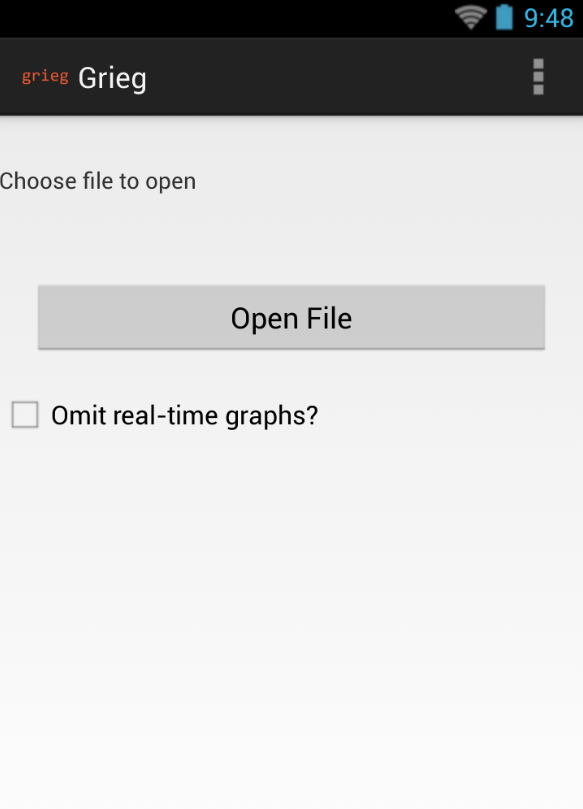
\includegraphics[width=7cm]{images/first_screen}

To ekran który użytkownik zobaczy od razu po uruchomieniu aplikacji. Dostaje on możliwość zaznaczenia opcji „Omit real-time graphs” oznaczającej wybranie ograniczonego \code{Pipeline} do wykresów które nie muszą być generowane w całości dla kolejnych fragmentów muzyki oraz dostaje możliwość wybrania pliku do analizy.

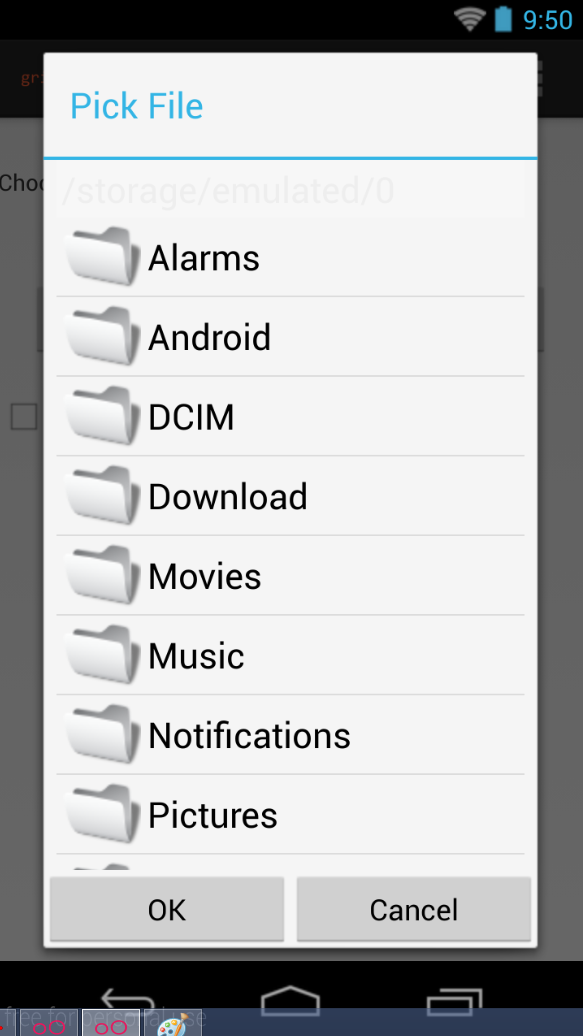
\includegraphics[width=7cm]{images/Pick_file}
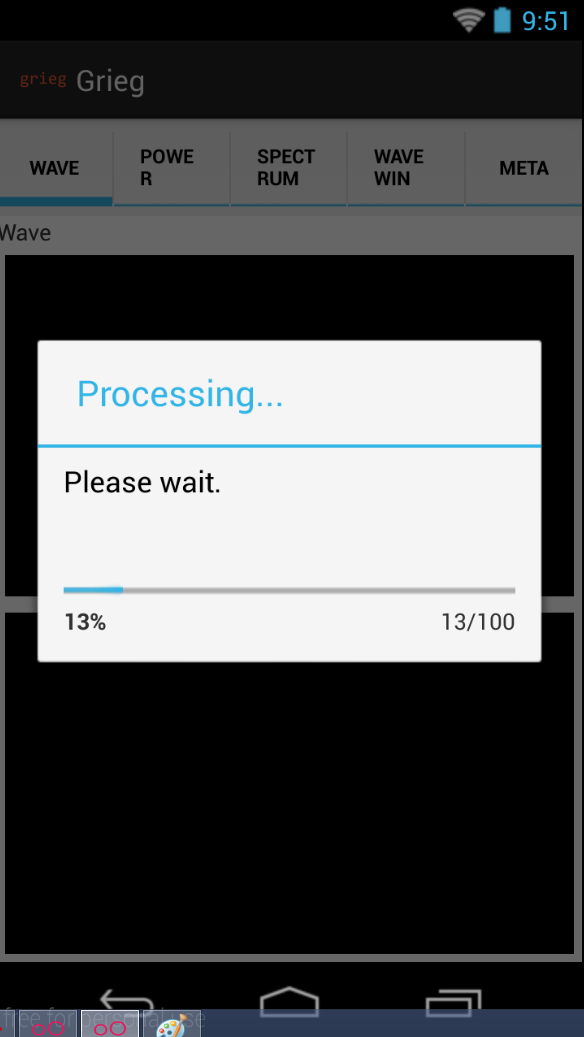
\includegraphics[width=7cm]{images/Processing}

Po wybraniu pliku przenosimy się na ekran główny który informuje nas o konieczności poczekania na analizę wstępną.

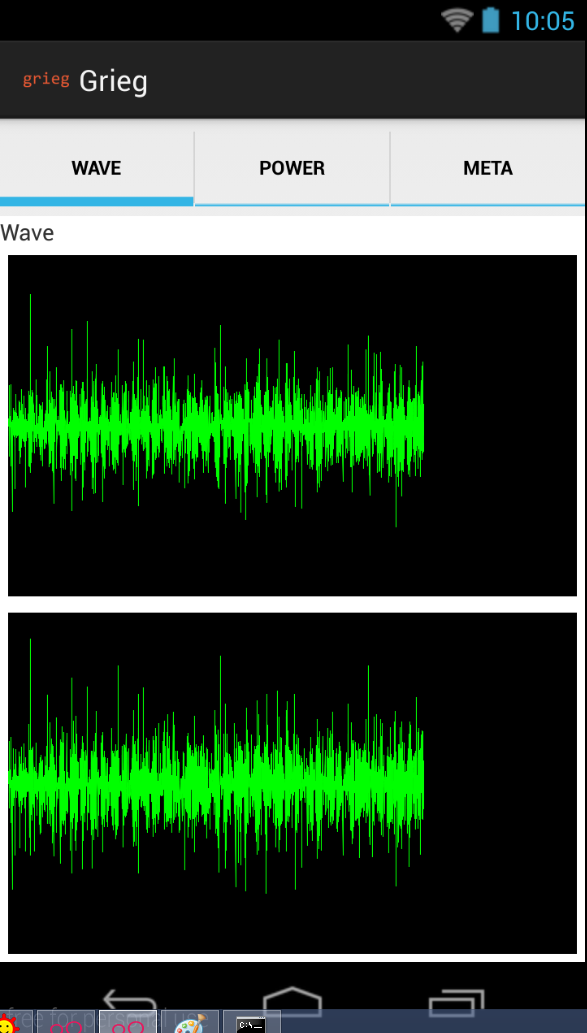
\includegraphics[width=7cm]{images/offline_wave_incomplete}

Gdy pre-analiza zostaje zakończona mamy dostęp do głównej części aplikacji. Widzimy tutaj wersję „niepełną” (tylko wykresy offline) na które składają się trzy zakładki - Wave (rysująca wykres fali dla dwóch kanałów), Power (rysująca wykres mocy fali dla dwóch kanałów) oraz Meta (zawierająca wczytane metadane). Jak widać wykresy rysowane są na oczach użytkownika z prędkością uzależnioną od mocy obliczeniowej urządzenia jak i długości utworu. Wykres mocy (czyli średniej kwadratowej amplitud próbek) jest analogiczny.

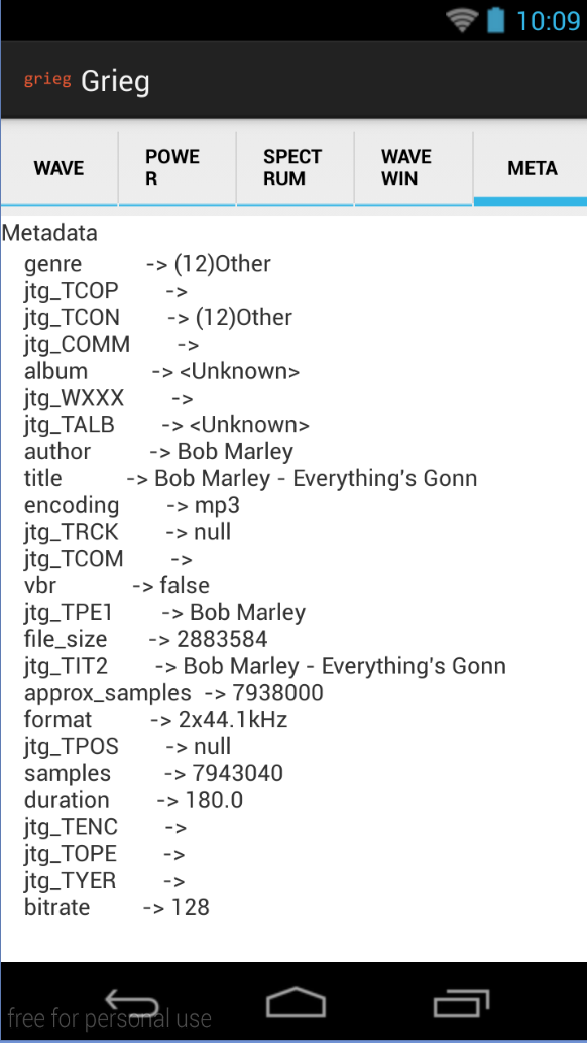
\includegraphics[width=7cm]{images/full_metadata}

Tutaj widzimy zakładkę metadanych wyświetlającą wszystkie informacje jakie zostały wyciągnięte (włącznie z tymi które nie zostały uzupełnione przez autora pliku). Plikiem tekstowym była piosenka Boba Marleya „Alright”. Autor został więc odnaleziony poprawnie, tak samo jak i tytuł (choć różny od poprawnego zgadza się z tym który został zapisany w pliku .mp3). Z ważniejszych informacji warto spojrzeć również na rozmiar pliku, przybliżoną liczbę sampli (potrzebną do odpowiedniego skalowania wyświetlania wykresów), czas trwania, Bitrate oraz format.
Warto też zauważyć że widzimy tutaj pełen zestaw zakładek - poza tymi które już widzieliśmy pojawiły się również „Spectrum” oraz „Wave win” które będą opisane poniżej.

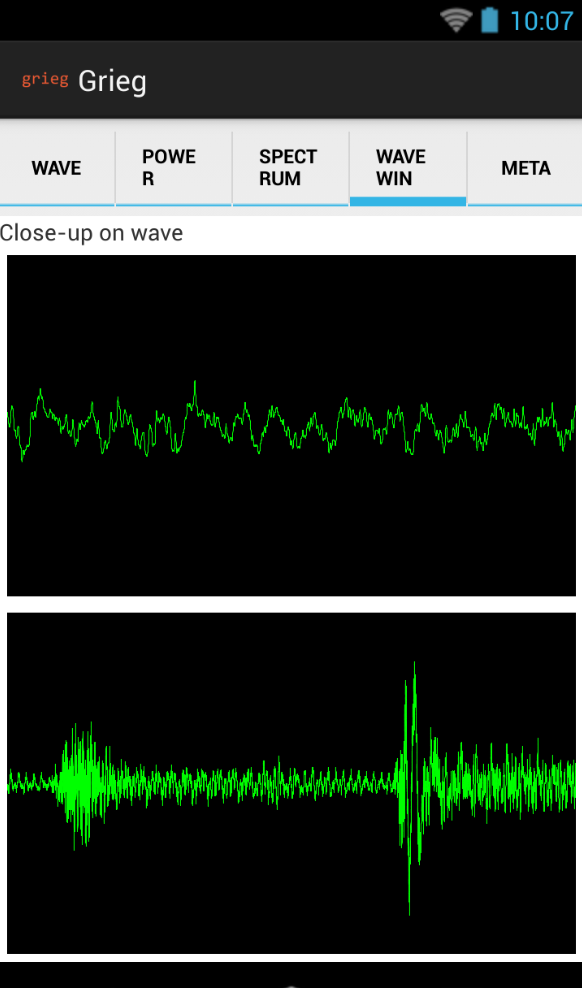
\includegraphics[width=7cm]{images/full_wave_window}

Zakładka „Wave win” rysuje, zgodnie z nazwą, okno fali w dwóch wersjach - szerokiej oraz wąskiej. Jest to wykres „online” w sensie potrzeby rysowania go dla każdego momentu utworu. Ze względu na ograniczenia wydajnościowe dzieje się to jednak rzadziej (około jednego obrazu na trzy-pięć sekund).

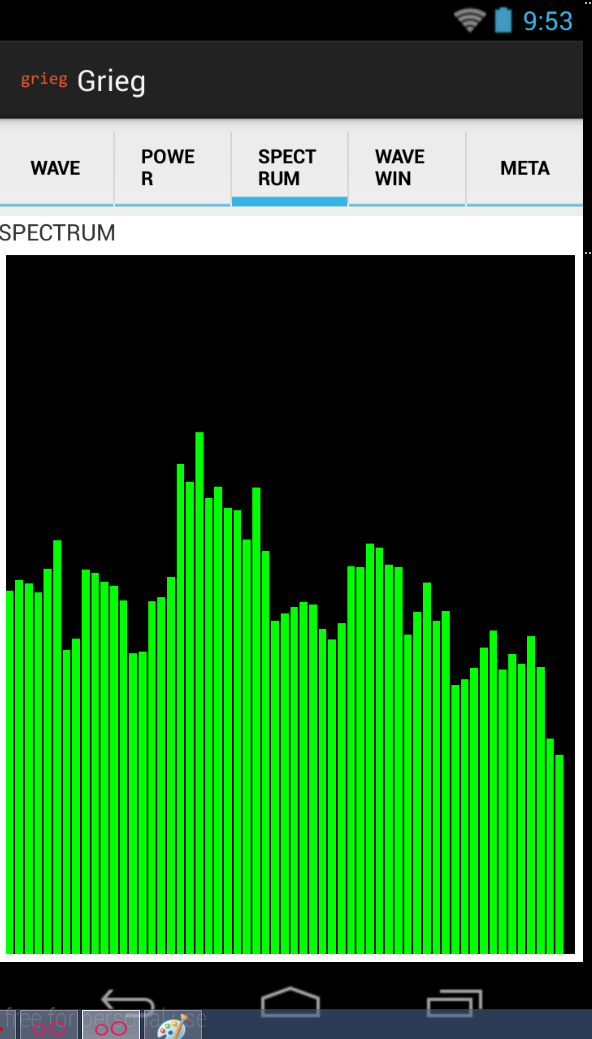
\includegraphics[width=7cm]{images/full_spectrum}

Ostatnim z wykresów jest wykres spektrum skonstruowany w znanej wielu ludziom formie „podskakujących prostokątów”. Jest to wykres natężenia poszczególnych częstotliwości w skali logarytmicznej na obydwu współrzędnych. Tak jak okno fali rysowany jest na żywo, w przeciwieństwie jednak do okna robi to efektywnie.

